%---------------------------------------------------
% Nombre: clustering.tex  
% 
% Texto del capitulo 1
%---------------------------------------------------

\chapter{Proceso exploratorio y pre-procesado}
\label{pre}

En este cap�tulo veremos el proceso seguido para afrontar y resolver el problema definido en puntos anteriores. El cap�tulo comienza detallando el proceso exploratorio inicial para continuar con el grueso de la memoria, la especificaci�n de los procesos de pre-procesado llevados a cabo y la soluci�n final aportada. 
 
\section{Proceso exploratorio}

En esta secci�n detallamos el proceso exploratorio seguido para obtener m�s informaci�n del problema y de los datos que tenemos entre manos. Los pasos seguidos en este proceso ser�an: 
\begin{enumerate}

\item \textbf{Tipos de datos y dimensiones}: El primer paso para enfrentarnos a los datos era conocer la dimensionalidad y el tipo de datos. Por ello, hicimos uso de los comandos \textbf{describe} y \textbf{str}, para comprobar como eran estos datos y sus distribuciones. Acotamos as� las variables num�ricas y los strings o factores que vimos en la tabla \ref{nonumericas}.

\item \textbf{Valores perdidos}: Al usar estudiar las distribuciones de los datos en el punto anterior descubrimos la existencia de valores perdidos en algunas variables. Para ver si este problema era muy acentuado se cre� una funci�n que nos ofrece el n�mero de valores perdidos de un dataset por variables con diversos estad�sticos. Tras obtener estos valores se representaron gr�ficamente para ver cuantos eran estos valores perdidos en funci�n de la variable y el conjunto de train (figura \ref{mvtrain}) o test (figura \ref{mvtest}).

\begin{figure}[H]
\centering
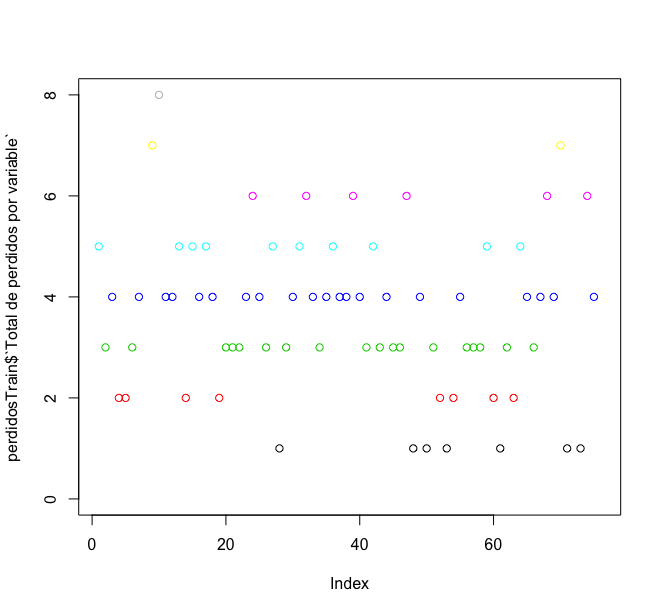
\includegraphics[width=10cm]{./Capitulo3/imagenes/mvtrain.png}
\caption{Distribuci�n de valores perdidos en train.}
\label{mvtrain}
\end{figure} 

Para comprobar la distribuci�n de valores perdidos y si se asemejan en n�mero en training y test, tambi�n se llevo a cabo un histograma (\ref{traintest}) conjunto que representa los valores perdidos en cada una de las particiones de datos. Este gr�fico nos llevo a comprobar que los valores perdidos \textbf{no siguen patrones} sino que son valores perdidos que parecen haber sido a�adidos aleatoriamente o pertenecer a fallos en la toma de datos. 

\begin{figure}[H]
\centering
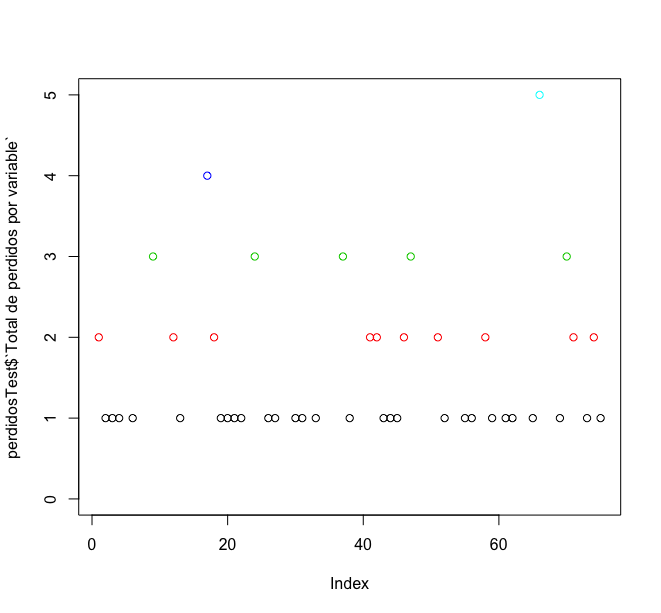
\includegraphics[width=8cm]{./Capitulo3/imagenes/mvtest.png}
\caption{Distribuci�n de valores perdidos en test.}
\label{mvtest}
\end{figure} 

\begin{figure}[H]
\centering
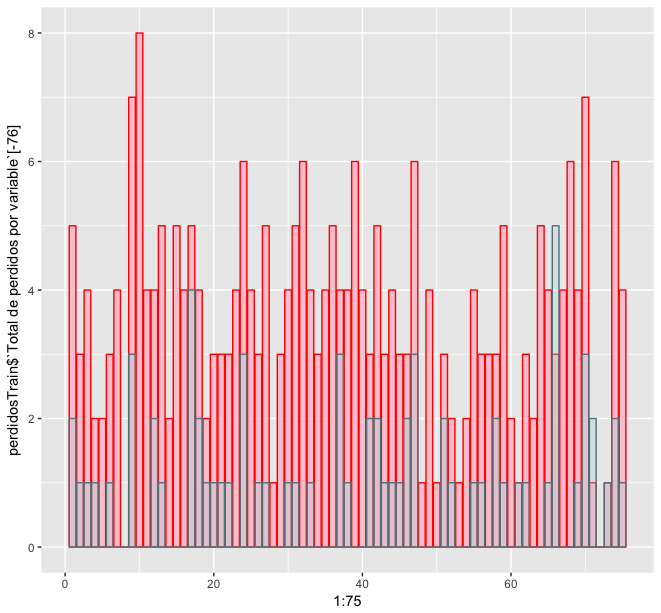
\includegraphics[width=9cm]{./Capitulo3/imagenes/traintest.png}
\caption{Distribuci�n de valores perdidos en train y test.}
\label{traintest}
\end{figure} 

\item \textbf{Correlaciones}: El tener tantas variables (75) y tanta presencia de valores perdidos hizo interesante la obtenci�n de correlaciones para comprobar si podemos eliminar variables en pos de otras o imputar los valores perdidos con los de otra variable muy correlada. Para ello, usamos la funci�n \textbf{corrplot}. El resultado podemos verlo en la figura \ref{correlacion} y descubrimos que la variable \textbf{x41} tiene correlacion de 1 con la \textbf{x48} siendo una el resultado del producto de la otra. 

\begin{figure}[H]
\centering
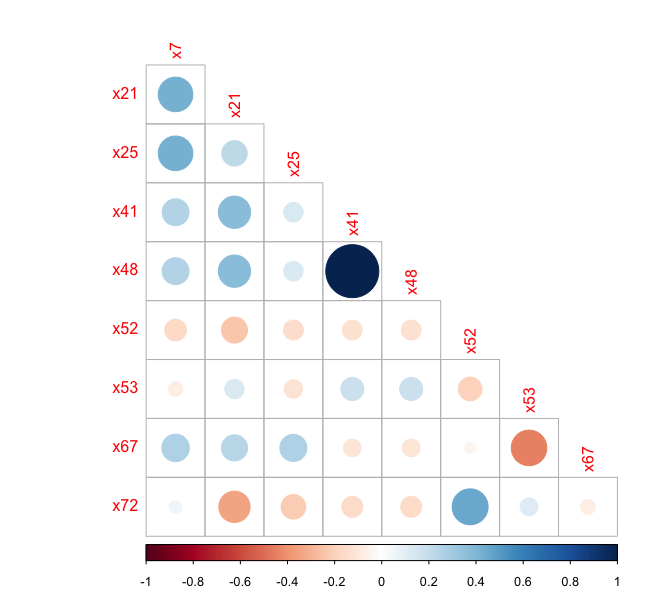
\includegraphics[width=9cm]{./Capitulo3/imagenes/correlacion.png}
\caption{Correlaci�n de variables.}
\label{correlacion}
\end{figure} 

\item \textbf{Outliers}: Dado el volumen del problema, se llev�  a cabo un estudio de outliers univariate b�sico basado en distancia intercuartil (IQR). Para que este proceso obtenga buenos resultados, se escalaron las variables y se analizaron solo aquellas cuyo dominio es continuo. Los resultados para las variables 1:30 pueden verse en el gr�fico \ref{130}  mientras que las variables 31:70 pueden verse en el gr�fico \ref{170}.

\begin{figure}[H]
\centering
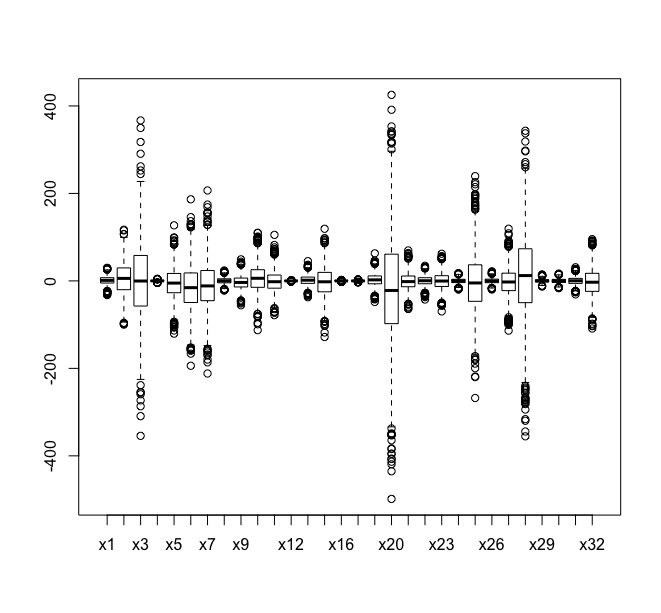
\includegraphics[width=8cm]{./Capitulo3/imagenes/130.png}
\caption{Boxplot de la primera mitad.}
\label{130}
\end{figure} 

\begin{figure}[H]
\centering
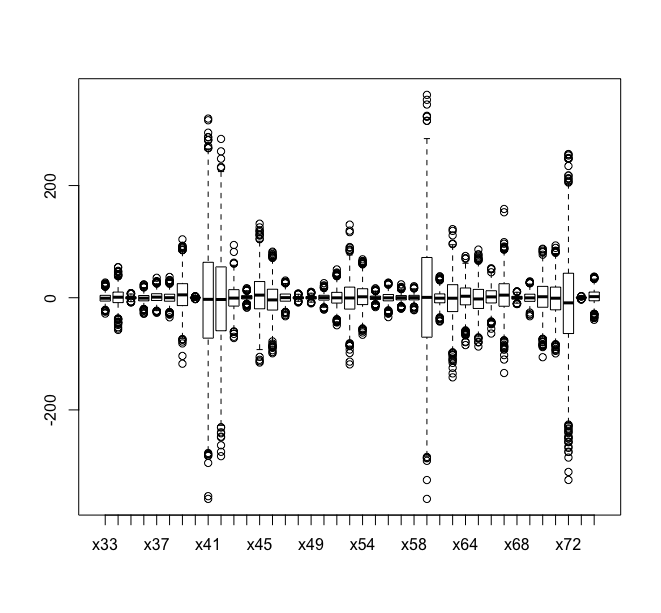
\includegraphics[width=8cm]{./Capitulo3/imagenes/170.png}
\caption{Boxplot de la segunda mitad.}
\label{170}
\end{figure} 

Tras el an�lisis de los boxplot podemos concluir que hay un gran n�mero de outliers, lo que nos lleva a pensar que probablemente estaremos ante un \textbf{dataset ruidoso} por lo que se deber� de probar t�cnicas de limpieza de ruido. 

\item \textbf{Distribuci�n clases}: Por �ltimo, en nuestro proceso de an�lisis exploratorio, se realiz� un gr�fico de distribuci�n de variables para comprobar si estamos ante un problema de clases balanceadas o en su defecto no balanceadas. El resultado puede verse en el gr�fico \ref{balanceadas}, donde queda constatado que estamos ante un problema donde la clase 0 y la 1 est�n en clara desventaja por lo que habr� que usar t�cnicas de \textbf{oversampling} o \textbf{undersampling}. 

\begin{figure}[H]
\centering
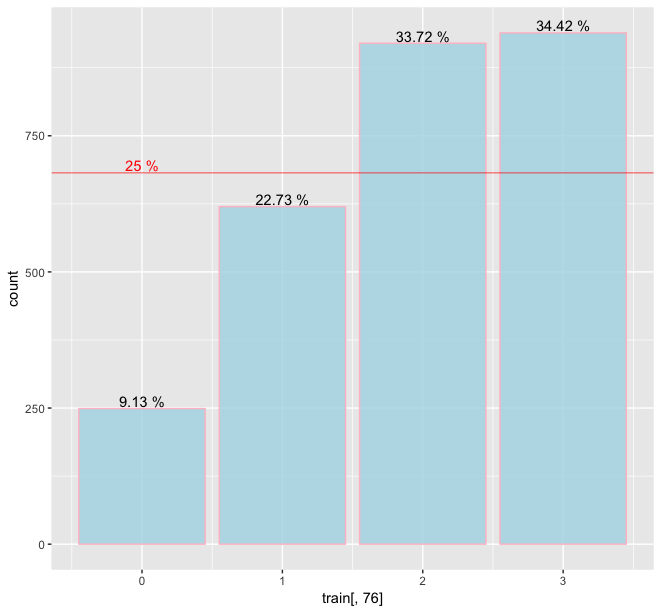
\includegraphics[width=8cm]{./Capitulo3/imagenes/balanceadas.png}
\caption{Distribuci�n de clases.}
\label{balanceadas}
\end{figure} 

\end{enumerate}

\section{Pre-procesado}

\section{T�cnicas de clasificaci�n}

\section{Soluci�n aportada}

\clearpage
%---------------------------------------------------